\documentclass[a4paper,12pt]{article}

\usepackage{paralist}
\usepackage[utf8x]{inputenc}
%\usepackage[T1]{fontenc}
\usepackage{eurosym}
\usepackage{fancyhdr}
\usepackage[italian]{babel}
\usepackage{url}
%\usepackage{lineno}
\usepackage{wrapfig}
\usepackage[pdftex]{graphicx}
%\usepackage{graphicx}
%\usepackage{sidecap}



\topmargin=0cm
\oddsidemargin=0cm
\evensidemargin=0cm
\textwidth=15cm
\textheight=21cm

%\headsep=-0.5cm
% \headheight=0cm

\pagestyle{fancyplain}
%\markboth{}


\headheight=1cm
% %\footskip=6cm
% \rhead[]{}
% \chead[]{\includegraphics[width=.8\textwidth]{vers_piccola_una_riga_nero.jpg}}
% %, \rhead, \lfoot, \cfoot and \rfoot

\lfoot{\medskip Andrea Trentini\\
andrea.trentini@unimi.it\\
Tel. +39 0250316274}
\cfoot{\hrule}
\rfoot{\medskip Dipartimento di Informatica\\
Via Comelico, 39\\
20135, Milano, Italy}

\title{\textbf{Proposta (2) per una serie di incontri su ``Arduino''}}
\author{Andrea Trentini}
%\date{Aprile 2015}

%%%%%%%%%%%%%%%%%%%%
%%%%%%%%%%%%%%%%%%%%
\begin{document}
\maketitle
\thispagestyle{fancy}
%\floatstyle{boxed}
%\restylefloat{figure}

\hspace{.30\textwidth}\textbf{Alla cortese attenzione di:}

\hspace{.40\textwidth}\textbf{Tatiana Cocca (sindaco)}
% tatiana.cocca@comune.cormano.mi.it

\hspace{.40\textwidth}\textbf{Marco Pilotti (assessore)}
% marco.pilotti@comune.cormano.mi.it

\hspace{.40\textwidth}\textbf{Fabrizio Vangelista (assessore)}
% fabrizio.vangelista@comune.cormano.mi.it

\hspace{.40\textwidth}\textbf{Annamaria Arcidiacono (ufficio stampa)}
%  annamaria.arcidiacono@comune.cormano.mi.it

\medskip

\hspace{.30\textwidth}\textbf{Comune di CORMANO}

\hspace{.30\textwidth}Piazza Scurati, 1

\hspace{.30\textwidth}20032 Cormano (MI)



% \tableofcontents
% \medskip
% \hrule


\section*{Introduzione}

In Luglio 2015 è stata organizzata una serata ``Arduino'' presso la Biblioteca 
comunale di Cormano. L'autore della presente era lo \textit{speaker}.
L'incontro è durato poco più di un paio d'ore e nonostante il caldo torrido 
(era il periodo di ``Acheronte'') la partecipazione si è attestata sulla 
cinquantina di persone coinvolte, attente e partecipative... tanto che la 
sessione domande e risposte ha preso circa metà della serata.

Molti degli astanti hanno espresso interesse per l'ipotesi di organizzare 
incontri periodici sul tema, qui di seguito una proposta di massima.

\section*{Serate ``Arduino''}

Ogni serata durerà un \textbf{paio d'ore}, la cadenza ideale è \textbf{una volta 
alla settimana} per un totale di \textbf{8/10 incontri}. Ogni incontro consterà 
di una parte iniziale di spiegazione cui seguirà un laboratorio guidato ed 
assistito. Nella seconda metà del ``corso'' ogni partecipante (o a gruppi) 
deciderà un progettino da realizzare e \textbf{presentare durante l'ultimo 
incontro}.

\textbf{Il taglio sarà assolutamente pratico e applicativo.}


\hrulefill

\textbf{Ipotesi giorno: GIOVEDI', dalle 21.00}


\hrulefill

\textbf{Ipotesi partenza corso: dal 29 ottobre 2015}


\hrulefill


Argomenti da trattare, in sequenza più o meno cronologica (non sono i titoli 
delle singole lezioni/incontri, ma i microargomenti che verranno trattati man 
mano):

\begin{enumerate}

\item installazione dell'IDE (Integrated Development Environment) l'ambiente 
di sviluppo, il software da installare sul proprio PC per sviluppare codice e 
farlo girare sull'Arduino

\item ciclo di sviluppo, fasi della programmazione: scrittura del codice, 
compilazione, caricamento su Arduino, esecuzione del programma

\item architettura di Arduino: caratteristiche delle varie versioni 
dell'hardware (da Arduino UNO fino a Arduino YUN/NUY), cenni di altre 
piattaforme analoghe (RaspberryPI, Beaglebone, Alix, Olimex, etc.)

\item il meccanismo base di funzionamento di Arduino: i metodi ``setup'' e 
``loop''

\item uso dell'IDE

\item trovare documentazione online

\item introduzione al linguaggio Wiring

\item variabili, espressioni, tipi di dato, operatori (``+'', ``-'', ``*'', 
etc.)

\item Input/Output attraverso le porte disponibili sulla scheda: come leggere 
informazioni da sensori e come attivare azioni sul mondo reale tramite attuatori

\item strutture di controllo (``if then else'', ``while'', ``for'', etc.)

\item definizione di funzioni

\item fondamenti di elettricità ed elettronica: tensioni, correnti, legge di 
Ohm, componenti passivi, etc.

\item esempi disponibili nell'IDE, librerie

\item gli shield: schede già pronte per funzionalità ormai standardizzate (es. 
motori in corrente continua e passo/passo, relè, rete ethernet, rete cellulare, 
wifi, bluetooth, etc.)

\item progetto finale... da un certo punto in poi si ``lavora'' sulle proprie 
idee


% \item Progetto finale
% 
% \item Progetto finale

\end{enumerate}


\section*{Partecipanti}

I requisiti per la partecipazione sono minimi: è sufficiente avere 
dimestichezza col computer (gestione file, uso corrente) e un po' di manualità 
(per trattare con la componentistica elettronica molto minuta).

Non vengono coinvolte tensioni elettriche pericolose per l'uomo mentre le 
operazioni ``pericolose'' (ad esempio la saldatura) avverrebbero sotto stretta 
assistenza e sorveglianza o addirittura eseguite solo dal docente.

L'unico rischio è rovinare la componentistica, che comunque non è molto costosa.


\section*{Materiale occorrente}

L'ideale sarebbe avere dei fondi per dotare il ``laboratorio'' di materiale, 
sia per l'uso comune che di uso esclusivo di ognuno dei partecipanti.

Per quanto riguarda la dotazione di \textbf{ogni partecipante} si tratterebbe 
in linea di massima di (con i costi approssimati):

\begin{itemize}
 \item un esemplare di scheda Arduino UNO \hfill 30 €
 \item un alimentatore (per far funzionare Arduino anche in autonomia) \hfill 
10 €
 \item un cavo USB \hfill 5 €
 \item una Breadboard \hfill 5 €
 \item un kit fili per la Breadboard \hfill 5 €
 \item in sala sovrebbe essere disponibile una presa di alimentazione per ogni 
postazione
 \item (varie da definire)
\end{itemize}

Invece per quanto riguarda il materiale di \textbf{uso 
collettivo} (quindi un solo esemplare) si potrebbero acquisire i seguenti:

\begin{itemize}
 \item Saldatore 30W  \hfill 30 €
 \item Stagno e ``pasta salda'' \hfill 10 €
 \item Abbondante componentistica varia (resistenze, condensatori, led, 
etc.) \hfill 25 €
 \item qualche shield Arduino (motor, ethernet, wifi, gsm, etc.) \hfill 
150 €
 \item altro da identificare \textit{in itinere}
\end{itemize}

Invece ogni partecipante dovrebbe provvedere per il PC, normalmente 
accollandosi il trasporto del proprio portatile. A meno che nella sede degli 
incontri non siano disponibili dei PC utilizzabili (devono avere connessione 
Internet e aver almeno una porta USB).

% \section*{Cos'è Arduino}
% 
% \hfill\url{http://arduino.cc}
% 
% \begin{wrapfigure}[10]{r}[10pt]{4cm}
% 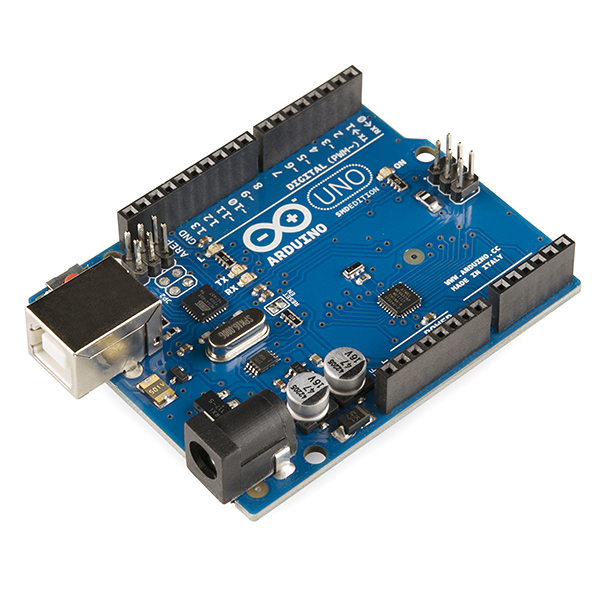
\includegraphics[width=4cm]{./Arduino_Uno_-_R3.jpg}
% \end{wrapfigure}
% 
% Arduino è un piccolissimo ``computer'' (per gli attuali standard di potenza di calcolo non avrebbe quasi diritto a questo rango, ma funzionalmente ha tutto ciò che serve per fare mini-applicazioni) inventato nel 2005 da un italiano, Massimo Banzi, per colmare una lacuna di allora.
% Mancava infatti in commercio una scheda per fare prototipi funzionanti che fosse semplice da usare, anche per i non informatici, e molto economica.
% 
% Banzi (insieme ai suoi colleghi all'Interaction Design Institute di Ivrea) progettò ciò che gli serviva e cominciò a distribuirlo con licenza libera\footnote{\url{http://it.wikipedia.org/wiki/Licenza_libera}}, sia l'hardware che il software erano liberamente accessibili: il software scaricabile gratuitamente, l'hardware disponibile a poco prezzo (poco più del costo di produzione).
% 
% Da allora l'ecosistema ``Arduino'' è letteralmente esploso: oggi sono disponibili moltissime versioni (per forma, dimensioni, potenza di calcolo, prezzo) del ``computer'' e una pletora di schede aggiuntive per realizzare sistemi ``embedded'' (autocontenuti), sensori (temperatura, umidità, luce, gas vari, inquinanti, accelerazione, campo magnetico, etc.) e attuatori (motori rotativi, passo-passo, relè).
% 
% Se oggi, termini come ``Internet of Things''\footnote{\url{http://it.wikipedia.org/wiki/Internet_delle_cose}} e ``Wearable computing''\footnote{\url{http://en.wikipedia.org/wiki/Wearable_computer}} sono noti al grande pubblico è anche (se non in gran parte) merito di Arduino.


% \section*{Perché organizzare un incontro su questo tema}
% 
% Qualunque appassionato di computer e di informatica ha sentito parlare di Arduino, ma non tutti hanno avuto occasione di vederne uno dal vivo, di provare a sviluppare una piccola applicazione, di capire come funziona e a cosa potrebbe essere utile nella vita di tutti i giorni.
% 
% Potrebbe essere interessante organizzare una serata (o un pomeriggio), un incontro di un paio d'ore al massimo in cui si potrebbe descrivere la piattaforma, fare una panoramica delle possibilità offerte e provare a realizzare lì per lì un'applicazione esemplificativa. Lo scopo è la diffusione di conoscenza, sconfiggendo la pigrizia mentale iniziale che magari fa dire alla propria testa ``lo farò domani'': sentire una persona che racconta e mostra cose è più semplice che mettersi a cercare materiale in rete (i.e., ``googlare''). Se poi l'interesse dovesse essere elevato nessuno vieta di organizzare altri incontri più ``operativi''.
% 
% In fondo i vicini di Cusano si sono già mossi: \url{http://www.sharemakers.it/}
% 
% %Il ``gap di ingresso'' () è bassissimo
% %piattaforma molto facile da affrontare/imparare, alla portata di tutti (sia in termini cognitivi che economici)
% 
% %usata per moltissime applicazioni



% 
% \section*{Chi sono e cosa faccio}
% 
% Sono ricercatore di Informatica presso l'Università di Milano, insegno ``Programmazione (Java)'', ``Cittadinanza Digitale \& Tecnocivismo''\footnote{\url{http://tecnocivismo.di.unimi.it/}} (un corso che trasmette ai nostri studenti la sensibilità verso gli aspetti politici/legali/sociali dell’informatica) e organizzo da alcuni anni degli appuntamenti periodici\footnote{\url{http://arduinoafternoon.di.unimi.it}} (circa due al mese) con studenti e appassionati esterni sul tema Arduino.
% 
% Milanese di nascita e Cormanese di adozione.
% 


\medskip
\hrule
\medskip
\medskip

\hfill Grazie, a presto!

\hfill Dott. Andrea Trentini

%\begin{figure}
% \centering
\hfill \includegraphics[width=5cm]{./Firma.png}
 % Firma.png: 640x320 pixel, 72dpi, 22.58x11.29 cm, bb=0 0 640 320
%\end{figure}



%%%%%%%%%%%%%%%%%%%%
\end{document}
